\begin{figure}[!hbp]
\centering
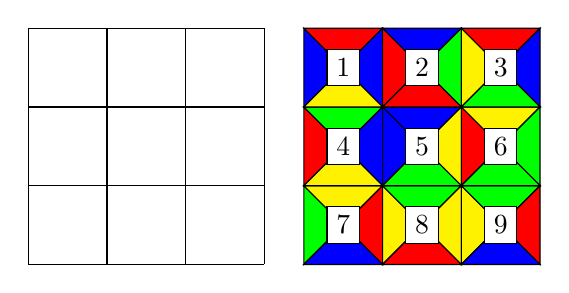
\begin{tikzpicture}
\draw (0,0) grid (3,3);

\draw[fill=green] (0 + 3.5, 0 + 0) -- (0 + 3.5, 0 + 1) -- (0 + 4, 0 + 0.5) -- cycle;
\draw[fill=yellow] (0 + 3.5, 0 + 1) -- (0 + 4.5, 0 + 1) -- (0 + 4, 0 + 0.5) -- cycle;
\draw[fill=red] (0 + 4.5, 0 + 1) -- (0 + 4.5, 0 + 0) -- (0 + 4, 0 + 0.5) -- cycle;
\draw[fill=blue] (0 + 3.5, 0 + 0) -- (0 + 4.5, 0 + 0) -- (0 + 4, 0 + 0.5) -- cycle;
\node[draw, fill=white] at (0 + 4, 0 + 0.5) {7};

\draw[fill=yellow] (1 + 3.5, 0 + 0) -- (1 + 3.5, 0 + 1) -- (1 + 4, 0 + 0.5) -- cycle;
\draw[fill=green] (1 + 3.5, 0 + 1) -- (1 + 4.5, 0 + 1) -- (1 + 4, 0 + 0.5) -- cycle;
\draw[fill=yellow] (1 + 4.5, 0 + 1) -- (1 + 4.5, 0 + 0) -- (1 + 4, 0 + 0.5) -- cycle;
\draw[fill=red] (1 + 3.5, 0 + 0) -- (1 + 4.5, 0 + 0) -- (1 + 4, 0 + 0.5) -- cycle;
\node[draw, fill=white] at (1 + 4, 0 + 0.5) {8};

\draw[fill=yellow] (2 + 3.5, 0 + 0) -- (2 + 3.5, 0 + 1) -- (2 + 4, 0 + 0.5) -- cycle;
\draw[fill=green] (2 + 3.5, 0 + 1) -- (2 + 4.5, 0 + 1) -- (2 + 4, 0 + 0.5) -- cycle;
\draw[fill=red] (2 + 4.5, 0 + 1) -- (2 + 4.5, 0 + 0) -- (2 + 4, 0 + 0.5) -- cycle;
\draw[fill=blue] (2 + 3.5, 0 + 0) -- (2 + 4.5, 0 + 0) -- (2 + 4, 0 + 0.5) -- cycle;
\node[draw, fill=white] at (2 + 4, 0 + 0.5) {9};

\draw[fill=red] (0 + 3.5, 1 + 0) -- (0 + 3.5, 1 + 1) -- (0 + 4, 1 + 0.5) -- cycle;
\draw[fill=green] (0 + 3.5, 1 + 1) -- (0 + 4.5, 1 + 1) -- (0 + 4, 1 + 0.5) -- cycle;
\draw[fill=blue] (0 + 4.5, 1 + 1) -- (0 + 4.5, 1 + 0) -- (0 + 4, 1 + 0.5) -- cycle;
\draw[fill=yellow] (0 + 3.5, 1 + 0) -- (0 + 4.5, 1 + 0) -- (0 + 4, 1 + 0.5) -- cycle;
\node[draw, fill=white] at (0 + 4, 1 + 0.5) {4};

\draw[fill=blue] (1 + 3.5, 1 + 0) -- (1 + 3.5, 1 + 1) -- (1 + 4, 1 + 0.5) -- cycle;
\draw[fill=blue] (1 + 3.5, 1 + 1) -- (1 + 4.5, 1 + 1) -- (1 + 4, 1 + 0.5) -- cycle;
\draw[fill=yellow] (1 + 4.5, 1 + 1) -- (1 + 4.5, 1 + 0) -- (1 + 4, 1 + 0.5) -- cycle;
\draw[fill=green] (1 + 3.5, 1 + 0) -- (1 + 4.5, 1 + 0) -- (1 + 4, 1 + 0.5) -- cycle;
\node[draw, fill=white] at (1 + 4, 1 + 0.5) {5};

\draw[fill=red] (2 + 3.5, 1 + 0) -- (2 + 3.5, 1 + 1) -- (2 + 4, 1 + 0.5) -- cycle;
\draw[fill=yellow] (2 + 3.5, 1 + 1) -- (2 + 4.5, 1 + 1) -- (2 + 4, 1 + 0.5) -- cycle;
\draw[fill=green] (2 + 4.5, 1 + 1) -- (2 + 4.5, 1 + 0) -- (2 + 4, 1 + 0.5) -- cycle;
\draw[fill=green] (2 + 3.5, 1 + 0) -- (2 + 4.5, 1 + 0) -- (2 + 4, 1 + 0.5) -- cycle;
\node[draw, fill=white] at (2 + 4, 1 + 0.5) {6};

\draw[fill=blue] (0 + 3.5, 2 + 0) -- (0 + 3.5, 2 + 1) -- (0 + 4, 2 + 0.5) -- cycle;
\draw[fill=red] (0 + 3.5, 2 + 1) -- (0 + 4.5, 2 + 1) -- (0 + 4, 2 + 0.5) -- cycle;
\draw[fill=blue] (0 + 4.5, 2 + 1) -- (0 + 4.5, 2 + 0) -- (0 + 4, 2 + 0.5) -- cycle;
\draw[fill=yellow] (0 + 3.5, 2 + 0) -- (0 + 4.5, 2 + 0) -- (0 + 4, 2 + 0.5) -- cycle;
\node[draw, fill=white] at (0 + 4, 2 + 0.5) {1};

\draw[fill=red] (1 + 3.5, 2 + 0) -- (1 + 3.5, 2 + 1) -- (1 + 4, 2 + 0.5) -- cycle;
\draw[fill=blue] (1 + 3.5, 2 + 1) -- (1 + 4.5, 2 + 1) -- (1 + 4, 2 + 0.5) -- cycle;
\draw[fill=green] (1 + 4.5, 2 + 1) -- (1 + 4.5, 2 + 0) -- (1 + 4, 2 + 0.5) -- cycle;
\draw[fill=red] (1 + 3.5, 2 + 0) -- (1 + 4.5, 2 + 0) -- (1 + 4, 2 + 0.5) -- cycle;
\node[draw, fill=white] at (1 + 4, 2 + 0.5) {2};

\draw[fill=yellow] (2 + 3.5, 2 + 0) -- (2 + 3.5, 2 + 1) -- (2 + 4, 2 + 0.5) -- cycle;
\draw[fill=red] (2 + 3.5, 2 + 1) -- (2 + 4.5, 2 + 1) -- (2 + 4, 2 + 0.5) -- cycle;
\draw[fill=blue] (2 + 4.5, 2 + 1) -- (2 + 4.5, 2 + 0) -- (2 + 4, 2 + 0.5) -- cycle;
\draw[fill=green] (2 + 3.5, 2 + 0) -- (2 + 4.5, 2 + 0) -- (2 + 4, 2 + 0.5) -- cycle;
\node[draw, fill=white] at (2 + 4, 2 + 0.5) {3};

\end{tikzpicture}
\caption{Un tablero de 3 x 3 con las fichas que se deben colocar en el tablero}
\label{ej_3:ej_1}
\end{figure}

\begin{figure}[!hbp]
\centering
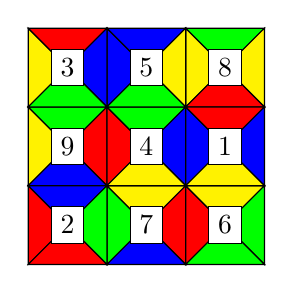
\begin{tikzpicture}

\draw[fill=green] (1 + 0, 0 + 0) -- (1 + 0, 0 + 1) -- (1 + 0.5, 0 + 0.5) -- cycle;
\draw[fill=yellow] (1 + 0, 0 + 1) -- (1 + 1, 0 + 1) -- (1 + 0.5, 0 + 0.5) -- cycle;
\draw[fill=red] (1 + 1, 0 + 1) -- (1 + 1, 0 + 0) -- (1 + 0.5, 0 + 0.5) -- cycle;
\draw[fill=blue] (1 + 0, 0 + 0) -- (1 + 1, 0 + 0) -- (1 + 0.5, 0 + 0.5) -- cycle;
\node[draw, fill=white] at (1 + 0.5, 0 + 0.5) {7};

\draw[fill=yellow] (2 + 0, 2 + 0) -- (2 + 0, 2 + 1) -- (2 + 0.5, 2 + 0.5) -- cycle;
\draw[fill=green] (2 + 0, 2 + 1) -- (2 + 1, 2 + 1) -- (2 + 0.5, 2 + 0.5) -- cycle;
\draw[fill=yellow] (2 + 1, 2 + 1) -- (2 + 1, 2 + 0) -- (2 + 0.5, 2 + 0.5) -- cycle;
\draw[fill=red] (2 + 0, 2 + 0) -- (2 + 1, 2 + 0) -- (2 + 0.5, 2 + 0.5) -- cycle;
\node[draw, fill=white] at (2 + 0.5, 2 + 0.5) {8};

\draw[fill=yellow] (0 + 0, 1 + 0) -- (0 + 0, 1 + 1) -- (0 + 0.5, 1 + 0.5) -- cycle;
\draw[fill=green] (0 + 0, 1 + 1) -- (0 + 1, 1 + 1) -- (0 + 0.5, 1 + 0.5) -- cycle;
\draw[fill=red] (0 + 1, 1 + 1) -- (0 + 1, 1 + 0) -- (0 + 0.5, 1 + 0.5) -- cycle;
\draw[fill=blue] (0 + 0, 1 + 0) -- (0 + 1, 1 + 0) -- (0 + 0.5, 1 + 0.5) -- cycle;
\node[draw, fill=white] at (0 + 0.5, 1 + 0.5) {9};

\draw[fill=red] (1 + 0, 1 + 0) -- (1 + 0, 1 + 1) -- (1 + 0.5, 1 + 0.5) -- cycle;
\draw[fill=green] (1 + 0, 1 + 1) -- (1 + 1, 1 + 1) -- (1 + 0.5, 1 + 0.5) -- cycle;
\draw[fill=blue] (1 + 1, 1 + 1) -- (1 + 1, 1 + 0) -- (1 + 0.5, 1 + 0.5) -- cycle;
\draw[fill=yellow] (1 + 0, 1 + 0) -- (1 + 1, 1 + 0) -- (1 + 0.5, 1 + 0.5) -- cycle;
\node[draw, fill=white] at (1 + 0.5, 1 + 0.5) {4};

\draw[fill=blue] (1 + 0, 2 + 0) -- (1 + 0, 2 + 1) -- (1 + 0.5, 2 + 0.5) -- cycle;
\draw[fill=blue] (1 + 0, 2 + 1) -- (1 + 1, 2 + 1) -- (1 + 0.5, 2 + 0.5) -- cycle;
\draw[fill=yellow] (1 + 1, 2 + 1) -- (1 + 1, 2 + 0) -- (1 + 0.5, 2 + 0.5) -- cycle;
\draw[fill=green] (1 + 0, 2 + 0) -- (1 + 1, 2 + 0) -- (1 + 0.5, 2 + 0.5) -- cycle;
\node[draw, fill=white] at (1 + 0.5, 2 + 0.5) {5};

\draw[fill=red] (2 + 0, 0 + 0) -- (2 + 0, 0 + 1) -- (2 + 0.5, 0 + 0.5) -- cycle;
\draw[fill=yellow] (2 + 0, 0 + 1) -- (2 + 1, 0 + 1) -- (2 + 0.5, 0 + 0.5) -- cycle;
\draw[fill=green] (2 + 1, 0 + 1) -- (2 + 1, 0 + 0) -- (2 + 0.5, 0 + 0.5) -- cycle;
\draw[fill=green] (2 + 0, 0 + 0) -- (2 + 1, 0 + 0) -- (2 + 0.5, 0 + 0.5) -- cycle;
\node[draw, fill=white] at (2 + 0.5, 0 + 0.5) {6};

\draw[fill=blue] (2 + 0, 1 + 0) -- (2 + 0, 1 + 1) -- (2 + 0.5, 1 + 0.5) -- cycle;
\draw[fill=red] (2 + 0, 1 + 1) -- (2 + 1, 1 + 1) -- (2 + 0.5, 1 + 0.5) -- cycle;
\draw[fill=blue] (2 + 1, 1 + 1) -- (2 + 1, 1 + 0) -- (2 + 0.5, 1 + 0.5) -- cycle;
\draw[fill=yellow] (2 + 0, 1 + 0) -- (2 + 1, 1 + 0) -- (2 + 0.5, 1 + 0.5) -- cycle;
\node[draw, fill=white] at (2 + 0.5, 1 + 0.5) {1};

\draw[fill=red] (0 + 0, 0 + 0) -- (0 + 0, 0 + 1) -- (0 + 0.5, 0 + 0.5) -- cycle;
\draw[fill=blue] (0 + 0, 0 + 1) -- (0 + 1, 0 + 1) -- (0 + 0.5, 0 + 0.5) -- cycle;
\draw[fill=green] (0 + 1, 0 + 1) -- (0 + 1, 0 + 0) -- (0 + 0.5, 0 + 0.5) -- cycle;
\draw[fill=red] (0 + 0, 0 + 0) -- (0 + 1, 0 + 0) -- (0 + 0.5, 0 + 0.5) -- cycle;
\node[draw, fill=white] at (0 + 0.5, 0 + 0.5) {2};

\draw[fill=yellow] (0 + 0, 2 + 0) -- (0 + 0, 2 + 1) -- (0 + 0.5, 2 + 0.5) -- cycle;
\draw[fill=red] (0 + 0, 2 + 1) -- (0 + 1, 2 + 1) -- (0 + 0.5, 2 + 0.5) -- cycle;
\draw[fill=blue] (0 + 1, 2 + 1) -- (0 + 1, 2 + 0) -- (0 + 0.5, 2 + 0.5) -- cycle;
\draw[fill=green] (0 + 0, 2 + 0) -- (0 + 1, 2 + 0) -- (0 + 0.5, 2 + 0.5) -- cycle;
\node[draw, fill=white] at (0 + 0.5, 2 + 0.5) {3};

\end{tikzpicture}
\caption{Soluci\'on colocando todas las fichas del problema de la figura \ref{ej_3:ej_1}}
\label{ej_3:ej_1_sol}
\end{figure}

